% RUN THE NEXT FEW LINES *BEFORE* KNITTING
% (MAKE SURE RNW OPTIONS ARE SET TO KNITR)

% setwd('/home/joebrew/Documents/uf/phc6016/assignment2')
% Sys.setenv(TEXINPUTS=getwd(),
%           BIBINPUTS=getwd(),
%           BSTINPUTS=getwd())

% \begin{filecontents*}{test.bib}
% 
% @article{Ogden2014,
%   doi= {10.1001/jama.2014.732},
%   url= {http://dx.doi.org/10.1001/jama.2014.732},
%   year = {2014},
%   month= {feb},
%   publisher= {American Medical Association ({AMA})},
%   volume= {311},
%   number= {8},
%   pages= {806},
%   author= {Cynthia L. Ogden and Margaret D. Carroll and Brian K. Kit and Katherine M. Flegal},
%   title= {Prevalence of Childhood and Adult Obesity in the United States, 2011-2012},
%   journal= {{JAMA}}
% }
% 
% 
% }
% \end{filecontents*}

%%%%%%%%%%%%%%%%%%%%%%%%%%%%%%%%%%%%%%%%%
% Journal Article
% LaTeX Template
% Version 1.3 (9/9/13)
%
% This template has been downloaded from:
% http://www.LaTeXTemplates.com
%
% Original author:
% Frits Wenneker (http://www.howtotex.com)
%
% License:
% CC BY-NC-SA 3.0 (http://creativecommons.org/licenses/by-nc-sa/3.0/)
%
%%%%%%%%%%%%%%%%%%%%%%%%%%%%%%%%%%%%%%%%%

%----------------------------------------------------------------------------------------
%  PACKAGES AND OTHER DOCUMENT CONFIGURATIONS
%----------------------------------------------------------------------------------------

\documentclass[twoside]{article}\usepackage[]{graphicx}\usepackage[]{color}
%% maxwidth is the original width if it is less than linewidth
%% otherwise use linewidth (to make sure the graphics do not exceed the margin)
\makeatletter
\def\maxwidth{ %
  \ifdim\Gin@nat@width>\linewidth
    \linewidth
  \else
    \Gin@nat@width
  \fi
}
\makeatother

\definecolor{fgcolor}{rgb}{0.345, 0.345, 0.345}
\newcommand{\hlnum}[1]{\textcolor[rgb]{0.686,0.059,0.569}{#1}}%
\newcommand{\hlstr}[1]{\textcolor[rgb]{0.192,0.494,0.8}{#1}}%
\newcommand{\hlcom}[1]{\textcolor[rgb]{0.678,0.584,0.686}{\textit{#1}}}%
\newcommand{\hlopt}[1]{\textcolor[rgb]{0,0,0}{#1}}%
\newcommand{\hlstd}[1]{\textcolor[rgb]{0.345,0.345,0.345}{#1}}%
\newcommand{\hlkwa}[1]{\textcolor[rgb]{0.161,0.373,0.58}{\textbf{#1}}}%
\newcommand{\hlkwb}[1]{\textcolor[rgb]{0.69,0.353,0.396}{#1}}%
\newcommand{\hlkwc}[1]{\textcolor[rgb]{0.333,0.667,0.333}{#1}}%
\newcommand{\hlkwd}[1]{\textcolor[rgb]{0.737,0.353,0.396}{\textbf{#1}}}%

\usepackage{framed}
\makeatletter
\newenvironment{kframe}{%
 \def\at@end@of@kframe{}%
 \ifinner\ifhmode%
  \def\at@end@of@kframe{\end{minipage}}%
  \begin{minipage}{\columnwidth}%
 \fi\fi%
 \def\FrameCommand##1{\hskip\@totalleftmargin \hskip-\fboxsep
 \colorbox{shadecolor}{##1}\hskip-\fboxsep
     % There is no \\@totalrightmargin, so:
     \hskip-\linewidth \hskip-\@totalleftmargin \hskip\columnwidth}%
 \MakeFramed {\advance\hsize-\width
   \@totalleftmargin\z@ \linewidth\hsize
   \@setminipage}}%
 {\par\unskip\endMakeFramed%
 \at@end@of@kframe}
\makeatother

\definecolor{shadecolor}{rgb}{.97, .97, .97}
\definecolor{messagecolor}{rgb}{0, 0, 0}
\definecolor{warningcolor}{rgb}{1, 0, 1}
\definecolor{errorcolor}{rgb}{1, 0, 0}
\newenvironment{knitrout}{}{} % an empty environment to be redefined in TeX

\usepackage{alltt}

\usepackage{lipsum} % Package to generate dummy text throughout this template
%\usepackage[style=apa,backend=biber]{biblatex}
%\usepackage[style=authordate, backend=biber]{biblatex-chicago}
%\usepackage[style=apa, backend=biber]{biblatex}
%\usepackage[backend=bibtex]{biblatex}
% \usepackage[
% backend=biber,
% style=alphabetic,
% sorting=ynt
% ]{biblatex}

\usepackage[sort, numbers]{natbib}
%\bibliographystyle{vancouver}
%\bibliography{xampl}
%\addbibresource{assignment2.bib}

\usepackage[sc]{mathpazo} % Use the Palatino font
%\usepackage{endnotes} % for placing notes at end of document
\usepackage[T1]{fontenc} % Use 8-bit encoding that has 256 glyphs
\linespread{1.05} % Line spacing - Palatino needs more space between lines
\usepackage{microtype} % Slightly tweak font spacing for aesthetics
%\usepackage{subfig} % for multiple figures/captions in one area
\usepackage[hmarginratio=1:1,top=32mm,columnsep=20pt]{geometry} % Document margins
\usepackage{multicol} % Used for the two-column layout of the document
\usepackage[hang, small,labelfont=bf,up,textfont=it,up]{caption} % Custom captions under/above floats in tables or figures
\usepackage{booktabs} % Horizontal rules in tables
\usepackage{float} % Required for tables and figures in the multi-column environment - they need to be placed in specific locations with the [H] (e.g. \begin{table}[H])
\usepackage{hyperref} % For hyperlinks in the PDF
\usepackage{lettrine} % The lettrine is the first enlarged letter at the beginning of the text
\usepackage{paralist} % Used for the compactitem environment which makes bullet points with less space between them
\usepackage{abstract} % Allows abstract customization
\renewcommand{\abstractnamefont}{\normalfont\bfseries} % Set the "Abstract" text to bold
\renewcommand{\abstracttextfont}{\normalfont\small\itshape} % Set the abstract itself to small italic text
\usepackage{titlesec} % Allows customization of titles
\renewcommand\thesection{\Roman{section}} % Roman numerals for the sections
\renewcommand\thesubsection{\Roman{subsection}} % Roman numerals for subsections
\titleformat{\section}[block]{\large\scshape\centering}{\thesection.}{1em}{} % Change the look of the section titles
\titleformat{\subsection}[block]{\large}{\thesubsection.}{1em}{} % Change the look of the section titles
\usepackage{fancyhdr} % Headers and footers
\pagestyle{fancy} % All pages have headers and footers
\fancyhead{} % Blank out the default header
\fancyfoot{} % Blank out the default footer
\fancyhead[C]{PHC 6016 $\bullet$ Social Epidemiology $\bullet$ Professor Catherine Striley} % Custom header text
\fancyfoot[RO,LE]{\thepage} % Custom footer text
%----------------------------------------------------------------------------------------
%	TITLE SECTION
%----------------------------------------------------------------------------------------

\title{\vspace{-15mm}\fontsize{24pt}{10pt}\selectfont\textbf{Childhood obesity as a social phenomenon}} % Article title

\author{
\large
\textsc{Joe Brew}\thanks{Dude / wannabe epidemiologist}\\[2mm] % Your name
\normalsize University of Florida \\ % Your institution
\normalsize \href{mailto:joebrew@gmail.com}{joebrew@gmail.com} % Your email address
\vspace{-5mm}
}
\date{}

%----------------------------------------------------------------------------------------
\IfFileExists{upquote.sty}{\usepackage{upquote}}{}
\begin{document}
%\SweaveOpts{concordance=TRUE}

\maketitle % Insert title

\thispagestyle{fancy} % All pages have headers and footers

%----------------------------------------------------------------------------------------
%	ABSTRACT
%----------------------------------------------------------------------------------------

% \begin{abstract}
% 
% \noindent \lipsum[1] % Dummy abstract text
% 
% \end{abstract}

%----------------------------------------------------------------------------------------
%	ARTICLE CONTENTS
%----------------------------------------------------------------------------------------

\begin{multicols}{2} % Two-column layout throughout the main article text

\section*{Introduction: }

\lettrine[nindent=0em,lines=3]{O}{besity} is a social phenomenon with physical manifestations. \\

It should come as no surprise that despite massive government efforts, the prevalence of childhood obesity in the United States shows no signs of decline \cite{Ogden2014} (see below chart).  American anti-obesity policies are largely \emph{personal} and/or \emph{medical}, with a focus on self-discipline, exercise, and confusing dietary guidelines.  \\

\begin{knitrout}
\definecolor{shadecolor}{rgb}{0.969, 0.969, 0.969}\color{fgcolor}

{\centering 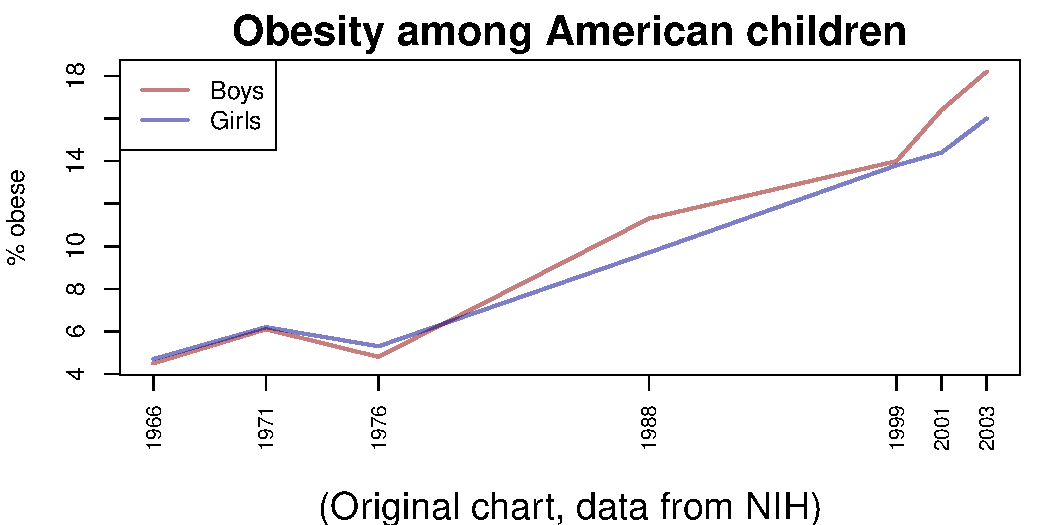
\includegraphics[width=\maxwidth]{figure/fig-plot1} 

}



\end{knitrout}
\cite{NIH}

Though the AMA took a step in the right direction by classifying obesity as a "disease" in 2013, %\cite{AMA}
the American public health and epidemiology community should take the next logical step by highlighting the nature of this disease as almost entirely \emph{social}.  If we begin to reframe the obesity epidemic in the context of its social determinants, we can begin to understand why medical and behavioral interventions at the individual level have such a poor track record. Non-social solutions to a social disease can hardly be expected to be effective. \\

What follows is an examination of recent literature on the social components of childhood obesity, followed by a brief personal reflection on the social components of the issue in Alachua County.

\section*{Literature: }

Obesity, at its core, is the result of simple thermodynamics: when the quantity of energy consumed is greater than energy expenditure the body stores the excess in the form of fat.  But studies suggest that both energy consumption and expenditure are largely conditioned by a multitude of social factors, including:\\

\textbf{Poverty} In the United States, poverty is positvely correlated with childhood obesity, even after adjustment for race \cite{Pan2012}.  Though the mechanisms by which poverty causes obesity are complex, theories range from the simple and intuitive (obesity-combatting products, such as gym memberships, come with a cost) to the more complex (poverty's correlation with violence creates a culture hositle to outdoor activities) \cite{Levine2011}.  \\

\textbf{Race} Conversely, even after adjustment for poverty, race is an independent risk factor for childhood obesity in the United States \cite{Ogden2014}.  This relationship is almost certainly not causal; rather, being black or hispanic is correlated with a number of other causal risk factors for obesity such as consumption of sugary bevarages, access to a television in the bedroom, and the introduction of solid foods (in lieu of breastfeeding) at an early age. \cite{Taveras2010}.  In some studies, statistically controlling for confounding factors yields no significant correlation between race and obesity \cite{Zilanawala2014}.   \\

\textbf{Peers and social norms} As anyone who has ever attended a Thanksgiving meal can tell you, our eating habits are conditioned by those around us.  A (relatively small) Dutch study found that children modified caloric intake directly as a result of those sitting near them at meal time \cite{Bevelander2012}.  As far as caloric expenditure, a New York City public school intervention resulted in increased physical activity during recess, even after the intervention had ended (though this study used highly subjective "visual scans" to quantify activity)  \cite{Chin2013}. \\

\textbf{Mistreatment} More recent studies shine light on the importance of behavioral and psychological factors in the development of childhood obesity.  Maternal depression during pregnancy appears to be an independent risk factor for overweight \cite{Taveras2010}.  Teasing appears to have a significant impact on childhood obesity, but uniquely among girls \cite{Feeg2014}. The psychological effects of mistreatment may be inter-generational: one study found that women who were maltreated as girls were more likely to undergo excessive gestational weight gain (which in turn is correlated with childhood obesity) \cite{Diesel2014}.

\section*{Alachua County}
Like other counties throughout the United States, social inequality in childhood health outcomes in Alachua are clear and persistent.  Last spring, using Alachua County Public Schools data for an internal FDOH report on childhood obesity in our county, I analyzed the correlation between race, poverty and obesity among area 6th graders. %\footnote{The reason for selecting sixth-graders was that all children go through a health screening which includes anthropometry upon entry into middle school.} \\

Though the direction of the result was unsurprising (being black or multiracial or qualifying for free/reduced lunch were risk factors for obesity), the magnitude and consistency of the effect was striking.  With every year's new generation of sixth graders, the differences between black/white children (left) and wealthy/poor (right) children were almost identical:\\

\vspace{2mm}
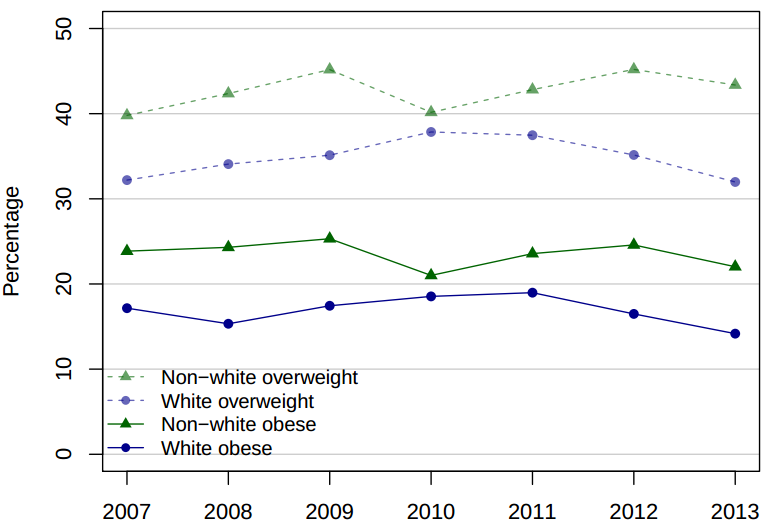
\includegraphics[height=70, width=110]{alachua2.png}
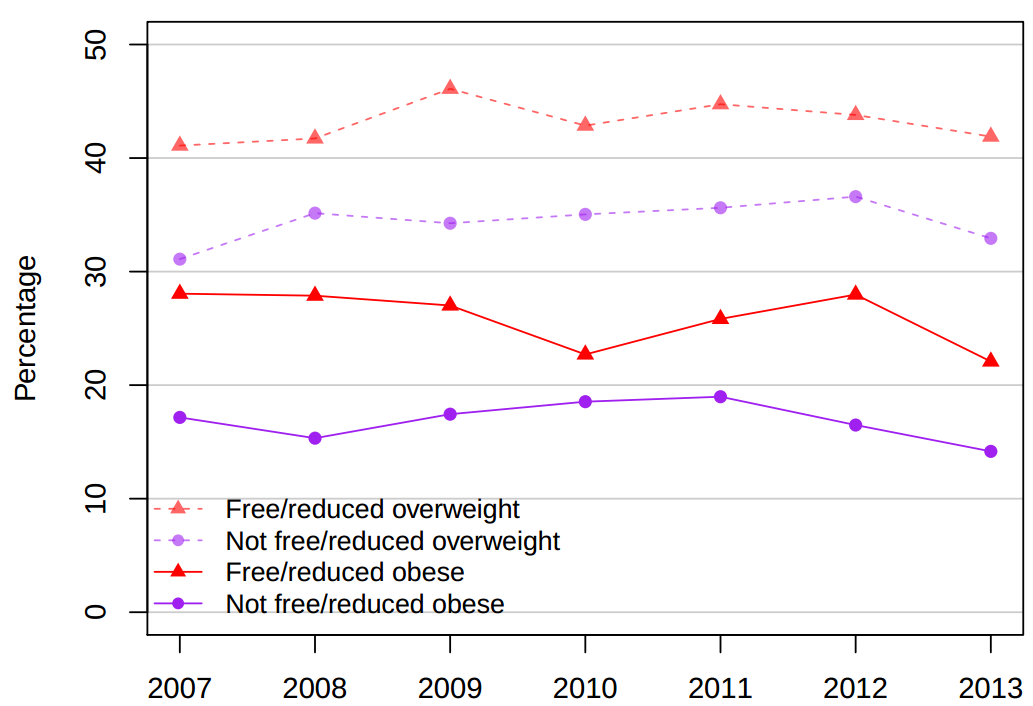
\includegraphics[height=70, width=110]{alachua4.png}
\vspace{2mm}


In other words, one could quite easily predict next year's prevalence of obesity by race and socioeconomic status.  Clearly these disparities were not the result of unpredictable human "choice" (true choice would have been far harder to predict) but rather underlying social currents to which we are all subject.

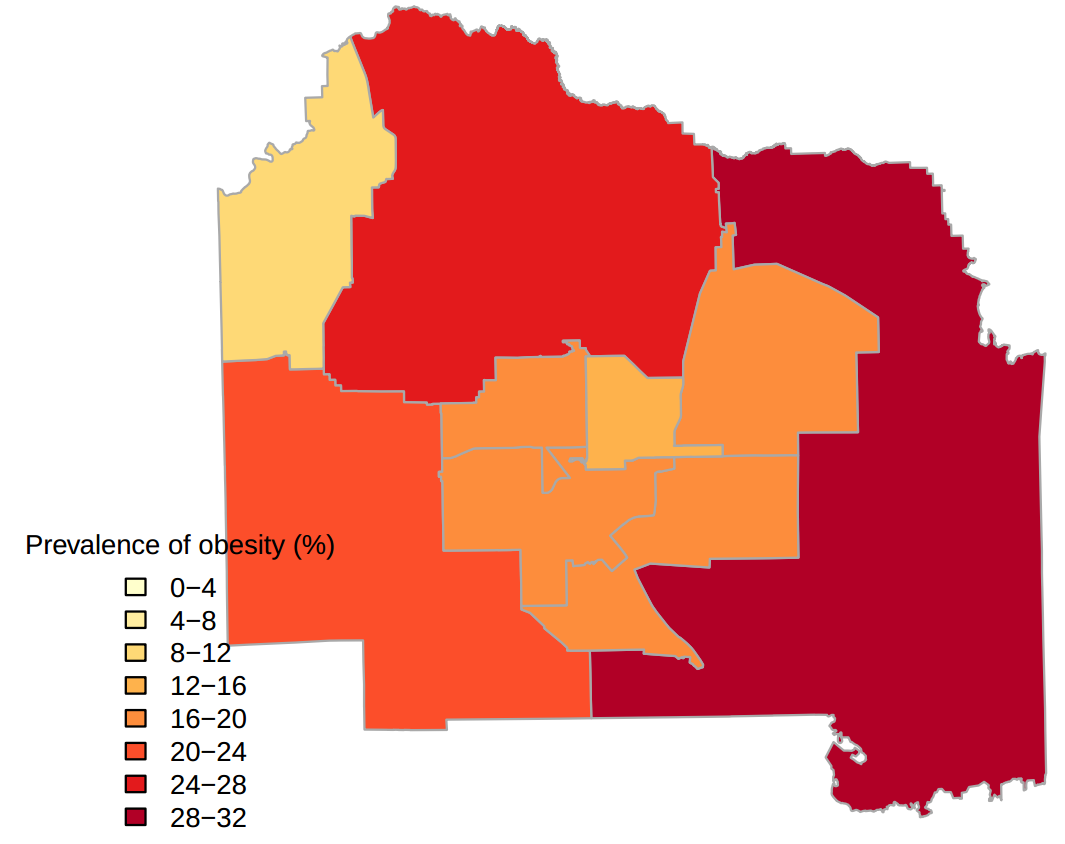
\includegraphics[height=120, width=165]{alachua3.png}


\section*{Conclusion}
The above map shows the prevalence of 6th grade obesity by school zone.  Sadly, it looks nearly identical to maps of dental caries, poverty, or absenteeism.  Like obesity, these are social illnesses with social solutions. But a lack of research into the \emph{causal pathways} of obesity hinders are potential to find these solutions.  The fetishization of personal responsibility, and the illusion of personal choice (particularly in the context of pediatric health) stand between us (public health practicioners) and effective interventions in the childhood obesity problem.  The evidence on obesity's social roots, some of which I have presented in the paper, is clear: our health hinges on the society we build together, not the choices we make alone.
%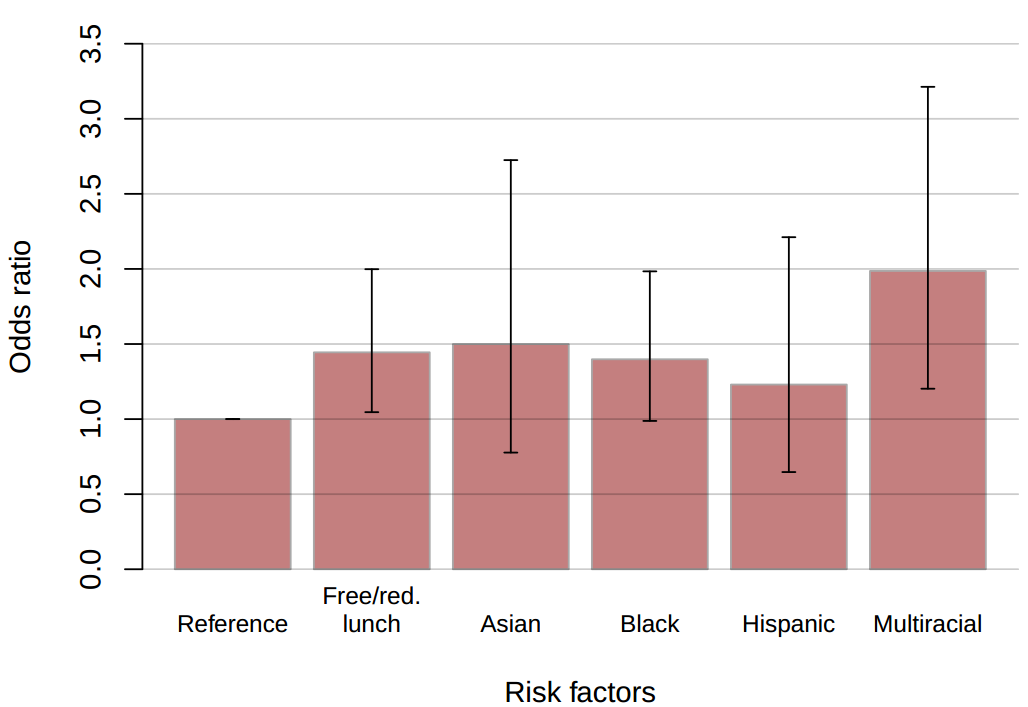
\includegraphics[height=140, width=200]{alachua.png}




%----------------------------------------------------------------------------------------
%	REFERENCE LIST
%----------------------------------------------------------------------------------------
\newpage
\bibliographystyle{unsrtnat}
\bibliography{test}

%----------------------------------------------------------------------------------------

\end{multicols}

\clearpage
\section*{Details}

\subsection*{Technical details} The entirety of this paper was written in Latex and the R programming languages.  The code for the production of this paper is available \href{https://github.com/joebrew/uf}{here}.  Below is information on the R session (in the interests of reproducibility):
\begin{knitrout}
\definecolor{shadecolor}{rgb}{0.969, 0.969, 0.969}\color{fgcolor}\begin{kframe}
\begin{verbatim}
## R version 3.0.2 (2013-09-25)
## Platform: x86_64-pc-linux-gnu (64-bit)
## 
## locale:
##  [1] LC_CTYPE=en_US.UTF-8       LC_NUMERIC=C              
##  [3] LC_TIME=en_US.UTF-8        LC_COLLATE=en_US.UTF-8    
##  [5] LC_MONETARY=en_US.UTF-8    LC_MESSAGES=en_US.UTF-8   
##  [7] LC_PAPER=en_US.UTF-8       LC_NAME=C                 
##  [9] LC_ADDRESS=C               LC_TELEPHONE=C            
## [11] LC_MEASUREMENT=en_US.UTF-8 LC_IDENTIFICATION=C       
## 
## attached base packages:
## [1] stats     graphics  grDevices utils     datasets  methods   base     
## 
## other attached packages:
## [1] knitr_1.6
## 
## loaded via a namespace (and not attached):
## [1] evaluate_0.5.5 formatR_1.0    stringr_0.6.2  tools_3.0.2
\end{verbatim}
\end{kframe}
\end{knitrout}

\end{document}
